\section{Coordination Approaches}
\subsection{Overview}
To be executable, each DSML defines a behavioral semantics. The specification of the behavior semantics of a DSML varies from natural language to the use of a formal language. In any case, the developing of complex applications relies on heterogeneous DSMLs thus resulting in heterogeneous behavioral models. In this context, Model coordination is a modeling approach to integrate the behavior of models. It proposes to specify the interaction between heterogeneous behavioral models by relying on a \emph{model of coordination}. According to \cite{coordsignibib}, ``\textit{Coordination is the process of building programs by gluing together active pieces}''. In this thesis, we adopt the wording of \emph{coordination} as being the explicit modeling of the interactions amongst behavioral models to obtain the emerging system behavior. In this sense, the coordination must be executable to enable the evaluation of the emerging behavior of the whole system. 
Coordination approaches have two major characteristics:
\begin{itemize}
	\item The interactions between models is defined separately from the computation of each model. 
	\item The individual behavior of models is kept while the coordination only constraints theirs behaviors. 
\end{itemize}
In this section, we present an overview of approaches that coordinate the behavior of models and languages. We categorize them into \emph{Coordination Languages and Architecture Description Languages}, and \emph{Coordination Frameworks}. The former enables a system designer to model the coordination between models whereas the latter provides a tool to automate the coordination of heterogeneous models by specifying the coordination between heterogeneous languages.

Coordination Languages have been proposed by Carriero et al.~\cite{coordsignibib} in order to model the coordination between heterogeneous behavioral models. Depending the entities coordinated, approaches can be categorized into \emph{data-driven} or \emph{control-driven}. The former coordinates data between models whereas the latter coordinates events between models. Arbab~\cite{whatdocoord} propose to classify the approaches into \emph{endogenous} and \emph{exogenenous} languages. An endogenous language provides coordination primitives that must be incorporated within a model for its coordination. For instance, Linda~\cite{lindabib} provides a set of primitives like \emph{in()} or \emph{out()} to exchange data between models. These primitives must be added to a host language by using libraries. Conversely, in exogenous coordination languages, the coordination is isolated from the models. General speaking, these approaches rely on the notion of interface that enables to homogenize the behavior of models. The coordination is specified between elements of the interface. Manyfold~\cite{manifoldbib} and Esper~\cite{esperbib} are control-driven and exogenous languages. More precisely, they rely on an interface made of events and the coordination is specified as constraint between those events. The main benefice of control driven exogenous languages is that enable a system designer to coordinate behavioral models without changing the current implementation.

In parallel, the \emph{software architecture} research field dealt with the growing complexity of software system by proposing languages (named ADL for Architecture Description Languages) to gain abstraction, structuring and reasoning capabilities~\cite{rapidebib,wrightbib,uniconbib,frameadlsbib,garlansoftarchbib}. An ADL usually specifies a system in terms of \emph{components} and interactions among those components. They enable a system designer to:
\begin{itemize}
	\item Clarify structural and semantics difference between components and interactions, 2) to reuse and compose architectural elements.
	\item Reuse and compose architectural elements.
	\item Identify/enforce commonly used patterns (\eg architectural styles).
\end{itemize}
Depending on the ADL, a \emph{Component} can for instance be an encapsulation of some procedure, an encapsulation of an object file or a (formal) abstraction of its behavior. To externally characterize the components, ADLs rely on well identified \emph{Component Interfaces}. The interfaces are used by \emph{Connectors} whose behavior is specified by a \emph{glue}. Connectors can represent a large variety of interactions (\eg procedure call, event broadcast or database queries) and the glue can range from a simple function to complex protocols. 

Both coordination languages and ADLs make a clear separation between two design activities: the specification of the component (\ie the computational aspects) and the assembly of these components (\ie the communication/coordination aspects). While the first activity is usually done by a software engineer, the second one is done by a system designer. He has to deal with the architecture-level communication that is expressed with complex protocols. To abstract away these protocols and make them reusable, ADLs propose connectors as types~\cite{frameadlsbib} that can be used on the shelf to specify domain specific interactions.

For example, Clara~\cite{clarabib} is an ADL dedicated to real time systems. It proposes built-in connector types like \emph{Rendez-vous}, \emph{Mutex} or \emph{Mailboxes}. This helps the task of a system designer by providing relevant domain specific connectors. However, this also limits what can appear in the interaction. 

Other approaches introduced the notion of \emph{user defined type}~\cite{uniconbib,wrightbib,reobib} that enables a system designer to build connectors for an specific domain. A connector type is defined by a set of \emph{roles} and a \emph{glue specification}. Roughly speaking, a role represents a formal parameter that is used to specify the glue. The glue is based on a formal language to specify how roles are coordinated. For instance, in Wright~\cite{wrightbib}, the glue is specified in a variant of CSP~\cite{csphoarebib}, whereas in Reo it is specified by the composition of dedicated primitives~\cite{reobib}. The connector types are later on instantiated and the roles are bound to the actual interfaces of the instances of components. 

\begin{figure}
	\begin{center}
		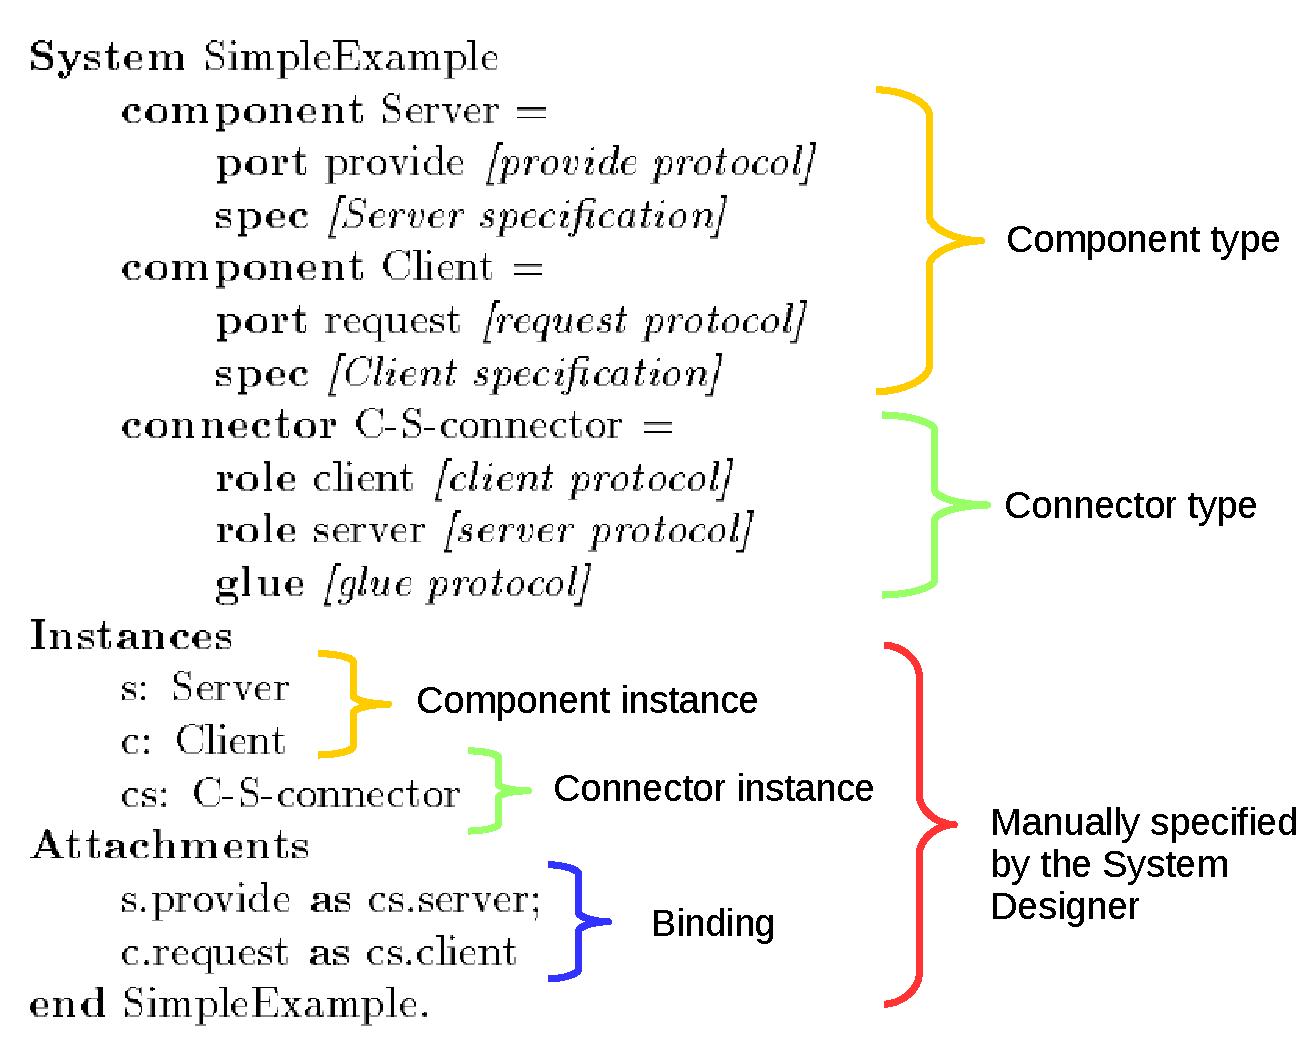
\includegraphics[width=0.5\textwidth]{background/figs/wrightspec}
		\caption{Specification of a Client-Server system in Wright~\cite{wrightbib}}
		\label{fig:wrightspec}
	\end{center}
\end{figure}

To illustrate how a system designer can define a set of domain specific connector types, Figure~\ref{fig:wrightspec} shows a simple client-server system described in Wright~\cite{wrightbib}. The specification defines two component types named \emph{Client} and \emph{Server}, and one connector type named \emph{C-S-connector}. The C-S-connector has two roles (\emph{client} and \emph{server}) and a glue that describes how the activities of the client and server roles are coordinated. The section \emph{Instances} describes a particular configuration by instantiating the corresponding components and connectors. The example describes a system where there is a single server (\emph{s}), a single client (\emph{c}) and a single connector (\emph{cs}). Then, the section \emph{Attachments} defines which component ports are attached to the connector roles. ADLs have successfully identified the need of connector types in order to ease the task of a system designer. In~\cite{wrightbib}, authors claim that connector types enables to ``\emph{understand a general pattern of interaction that can occur many times in any given system}''. Thus, a system designer has only to instantiate and bind connector types as needed by its architecture. 

The major drawback of coordination languages and ADLs is that the specification of the coordination is between particular models. For example, in the case of ADLs, a system designer has to instantiate and bind connector types manually. Returning to the example of Figure~\ref{fig:wrightspec}, for each server and client in the system, the system designer has to instantiate two components and one connector. Then, he has to bind the component ports with the connector roles. With the increasing number and heterogeneity of the components, this task can quickly become difficult and error prone.

\emph{Coordination Frameworks} identified that the instantiation and binding of connector types can be a systematic activity the system designer repeats many times and can consequently be defined as a pattern. Such a pattern is based on the \emph{know-how} of the system designer and sometimes on naming or organizational conventions adopted by the models. Thus, they have captured the specification of a \emph{behavioral coordination pattern} inside a tool/framework to automate the instantiation and binding of connector types. In these approaches, the coordination is specified between heterogeneous languages rather than between particular models. 
\begin{figure}
	\begin{center}
		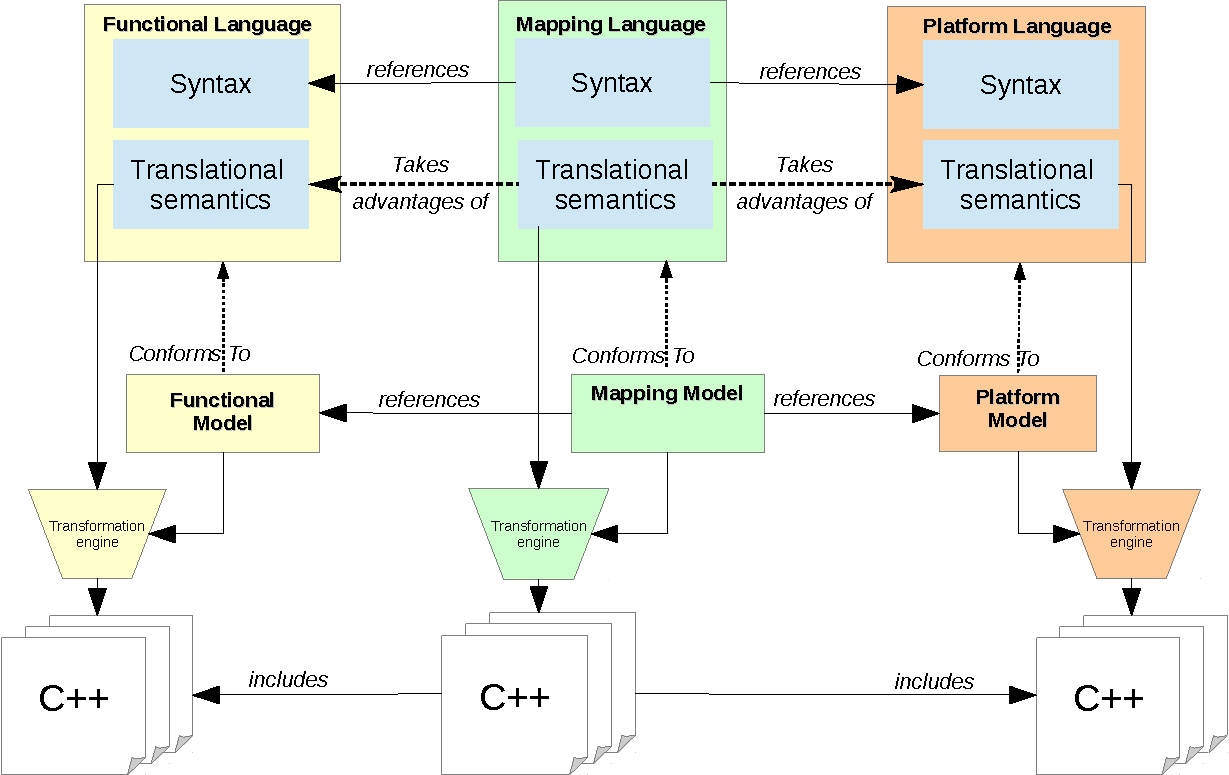
\includegraphics[width=0.7\textwidth]{background/figs/diNatale}
		\caption{High Level view of the approach proposed by Di Natale et al. in~\cite{dinatale}}
		\label{fig:diNatale}
	\end{center}
\end{figure}
% maltab and sdl has a sintax but also a semantics coompletly different. 
% matlab is data flow (sdf) y sdl (control flow or fsm)
% matlab vectores de datos, sdl events. 
% implementa como sincronizar eventos con datos

For example, MASCOT~\cite{mascotbib} is an approach focused on the integration of Matlab~\cite{matlabbib} and SDL~\cite{sdlbib}. Whereas SDL is a language suitable for control systems modeling, Matlab is better for modeling dataflow aspects of a system. However, these languages are very different, while SDL processes operate on events, represented by simple signals, Matlab processes operate on vectors, represented by vectorized signals. Thus, authors propose to automate the synchronization of control signals from SDL with data signals from Matlab. These signals can be either notification signals or message signals. Notification signals do not carry a value and are used to notify a process that an event has occurred. Message signals carry a value and are used to indicate a change of some variable or parameter. The approach deals with the integration of the timing and synchronization concepts from both languages by proposing two synchronization modes: head synchronization and tail synchronization. These mechanisms take advantages of the knowledge about the semantics of the languages. For instance, in the head synchronization, when a model in matlab receives a frame \emph{a1}, it immediately transforms \emph{a1} into \emph{b1} (dataflow network model). Any control signal from SDL that occurs during the transformation of \emph{a1} to \emph{b1} cannot influence its value. Then, the head synchronization mode ensures that the occurrence of the control signal is taken into account when the next frame is processed. In the tail synchronization, when a model in Matlab receives a control signal from SDL, the signal is collected until it cease to occur, then, it is translated to a vector and passed to the Matlab model. The modes of synchronization ensure the communication between Matlab and SDL. In addition, the approach gives a set of guidelines to aid the system designer to choose between the two synchronization proposed. Once the synchronization policy is defined, the approach enables the co-simulation of a SDL model and a Matlab model. The implementation is based on SDL wrappers. A process in the SDL specification that is specified in Matlab contains a wrapper that interfaces between the SDL simulator and the Matlab engine. A SDL wrapper is made of a set methods that enable the SDL engine to control the behavior of the data signals in Matlab. To do so, the approach relies on the name of signals in SDL specification to communicate with the signals in Matlab. The approach thus forces the system designer to follow a naming convention between signals in both domains. Although the current implementation partially automates the coordination of signals from both domains, the approach has identified and captured a coordination pattern between a control-flow language and a data-flow language by relying on some knowledge about its syntax and semantics.

In~\cite{dinatale}, authors deal with the integration of a language to describe the functional aspects and a language to describe the platform by proposing a dedicated mapping language. The mapping language syntax references syntactic elements from both the functional and the platform language. For instance, the $SWdeployment$ concept from the mapping model, references the $Task$ concept from the functional model and the $CPU$ concept from the platform model. Based on the mapping model, the approach generates the code of the communication between the functional and platform models. The semantics of both the functional and the platform language is defined by an translational approach into C++ code. The translational semantics of the mapping language takes advantages of some knowledges about the translational semantics of the other languages. For instance, for each subsystem in the functional language, authors know that a class is generated with name \emph{SubsystemName}\texttt{ModelClass}. They also know that the class has a \texttt{step} operation for the runtime evaluation of the block outputs given the inputs and the state. Thus, from a mapping model, the approach can generate the code to communicate a functional and platform model. The approach proposes a set of connectors that the system designer has to instantiate in the mapping model. In this sense, it is similar than others ADLs that propose a set of built-in connectors. However, different than other ADLs, connectors types link concepts from the syntax of languages. In particular, these connectors capture some knowledge of a system designer that performs the mapping of a functional model to a platform model. 
 
%The semantics of both the functional and the platform language is defined by an translational approach into C++ code. 

%This approach has achived to: 1) propose a dedicated language to explicitly relate concepts from both languages. Such a language contains as a built-in connector types that the developer can instantiate. 2) From such connectors, a generative approach enables to generate the comunication code in C++. 



%A first interesting aspect of this approach comes from the possibility, by creating a dedicated language, to reuse existing languages, and based on a mapping model to automatically generate the glue between the implementation of the models (in this case encoded in C++). 

%The mapping language syntax references syntactic elements from both the functional and the platform language. For instance, the $SWdeployment$ concept from the mapping model, references the $Task$ concept from the functional model and the $CPU$ concept from the platform model. 


%The translational semantics of the mapping language takes advantages of some knowledges about the translational semantics of the other languages. For instance, for each subsystem in the functional language, authors know that a class is generated with name \emph{SubsystemName}\texttt{ModelClass}. They also know that the class has a \texttt{step} operation for the runtime evaluation of the block outputs given the inputs and the state. 

%In other words, authors have a partial but sufficient knowledge of the translational semantics of both the functional and the platform language. 

%Finally, based on this knowledge, they encode in the translational semantics the glue to generate according to the actual mapping in the mapping model. 

 \begin{figure}
 	\begin{center}
 		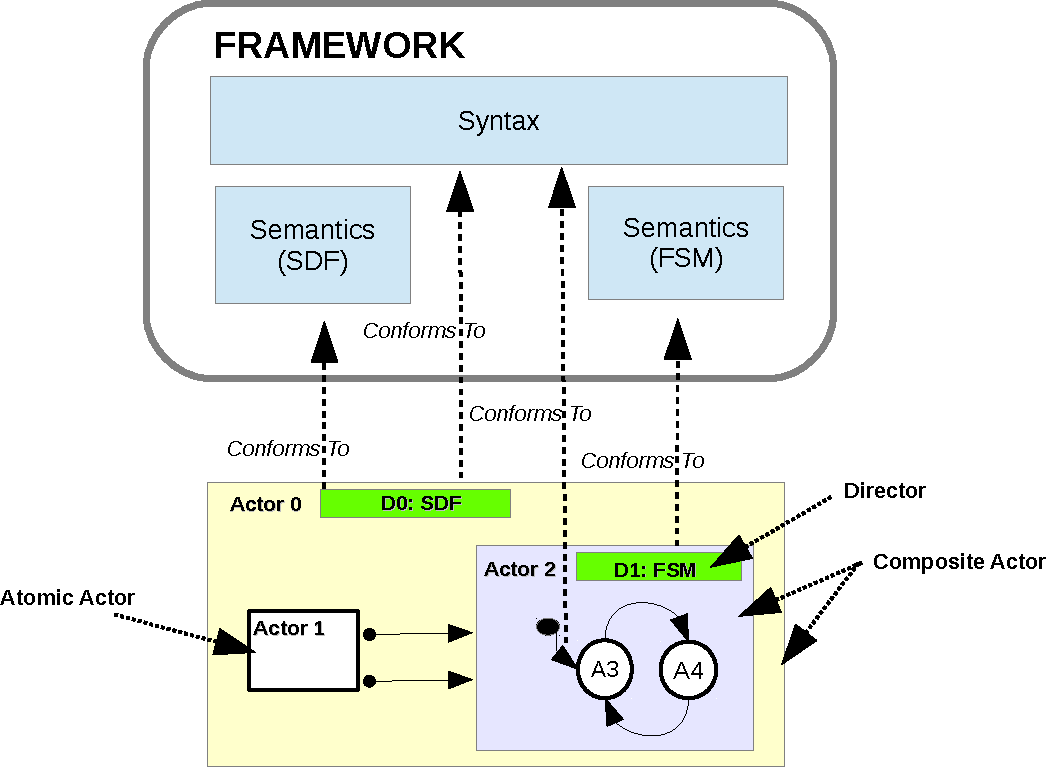
\includegraphics[width=0.7\textwidth]{background/figs/ptolemyfig}
 		\caption{High level view of Ptolemy~\cite{giraultbib}}
 		\label{fig:ptolemyfig}
 	\end{center}
 \end{figure}
 
 While the previous approaches are ad-hoc solution for two particular languages, Ptolemy~\cite{ptoleframebib} and ModHel'X~\cite{modhelxbib} are systematic approaches to coordinate models that conform to a set of predefined languages. These approaches rely on framework in which the syntax of models is described by actors and the semantics is given by a Model of Computation (MoC). Actors can be atomic (\eg \emph{Actor 1} in Figure~\ref{fig:ptolemyfig}) or composite (\eg \emph{Actor 0} and \emph{Actor 2} in Figure~\ref{fig:ptolemyfig}), \ie made of internal actors. Each composite actor has associated a model of computation that defines a \emph{Domain}. A domain specifies the communication semantics and the execution order among internal actors. A domain is implemented by a \emph{Director}. For instance, in Figure~\ref{fig:ptolemyfig}, the \emph{Actor 0} has the director \emph{D0} that follows the semantics of SDF and the \emph{Actor 2} has the director \emph{D1} that follows the semantics of FSM. In this approach, actors, both atomic and composite, are executable. In a composite actor, the execution order of internal actors is controlled by a director. In the example of Figure~\ref{fig:ptolemyfig}, the director \emph{D0} controls the execution of the \emph{Actor 1} and \emph{Actor 2} and director \emph{D1} controls the execution of \emph{A3} and \emph{A4} whenever \emph{Actor 2} is executed. In this sense, the execution of composite actors is strictly hierarchical. The behavior of actors is represented by a generic interface that contains a set of methods, \eg fire(). The MoC implemented by the director of a composite actor specifies when the methods in the interface of internal actors are invoked. For instance, when a composite actor is fired, the director associated with the composite actor fires the actors of the contained model. Based on a fixed syntax and a generic interface, these approaches have achieved to capture a hierarchical coordination pattern into a framework. The framework provides a dedicated syntax to specified the pattern, \ie composite actors, and encodes the necessary glue between interfaces to coordinate their execution. 
 
\subsection{Discussion}
Coordination languages and ADLs enable the system designer to define one or more models of coordination to specify how behavioral models interact. The main benefice of these approaches is that the global behavior is explicit and amenable for reasoning (for instance for Verification and Validation activities). Furthermore, they propose languages closed to system designer domain. For example, ADLs provide types in order to define domain specific connectors.  

These approaches have successfully identified connectors type, however, a system designer has still to specify when a type of connectors is used. He has to manually instantiate them by relying on his know-how. In a complex system, such a task can quickly become tedious and error prone. Furthermore, if one of the model changes, the model of coordination must also be changed. By relying on Coordination Languages and ADLS, a system designer only captures the solution for one single problem but he is not able to specify a systematic way to coordinate models. 

Conversely, Coordination frameworks have achieved to capture the know-how of a system designer by specifying coordination patterns. Such specification at language level allows automating the coordination between behavioral models. However, they embed the coordination pattern inside a tool. This has two major drawbacks:
\begin{itemize}
	\item 1) Validation and verification activities are limited since the coordination is encoded by using a general purpose language (\eg Java in Ptolemy and ModHel'X).
	\item 2) The system designer cannot change the proposed coordination without altering the core of the tool. 
\end{itemize} 
Regarding the point number one, coordination languages have already talcked this problem by using a formal language to express the coordination (\eg CSP in Wright). This enables providing verification and validation of the coordinated system. Recent work in that direction is presented in~\cite{semanticadaptccsl} where CCSL~\cite{ccslbib} is used to specify the semantic adaption in ModHel'X. 

Concerning the point number two, for complex systems, the system designer may need to capture several coordination patterns and potentially combine them. However, current coordination frameworks can only support such a variation by modifying the framework itself. The coordination model is mixed with the functional model, which makes it very tricky to modify one without risking altering the other.

To summarize, the achievement of coordination approaches are:
\begin{itemize}
	\item To become the interaction between behavioral models explicit and formal. 
	\item To leverage on the system designer know-how by capturing coordination patterns. 
\end{itemize}